The CML compiler has as \emph{input},
source files defined using its own conceptual language (as specified in this document),
which provides an abstract syntax similar to (but less comprehensive than) a combination of UML \cite{uml} and OCL \cite{ocl};
and, as \emph{output}, any target languages based on extensible templates,
which may be provided by the compiler's base libraries, by third-party libraries, or even by developers.

\begin{figure}
\centering
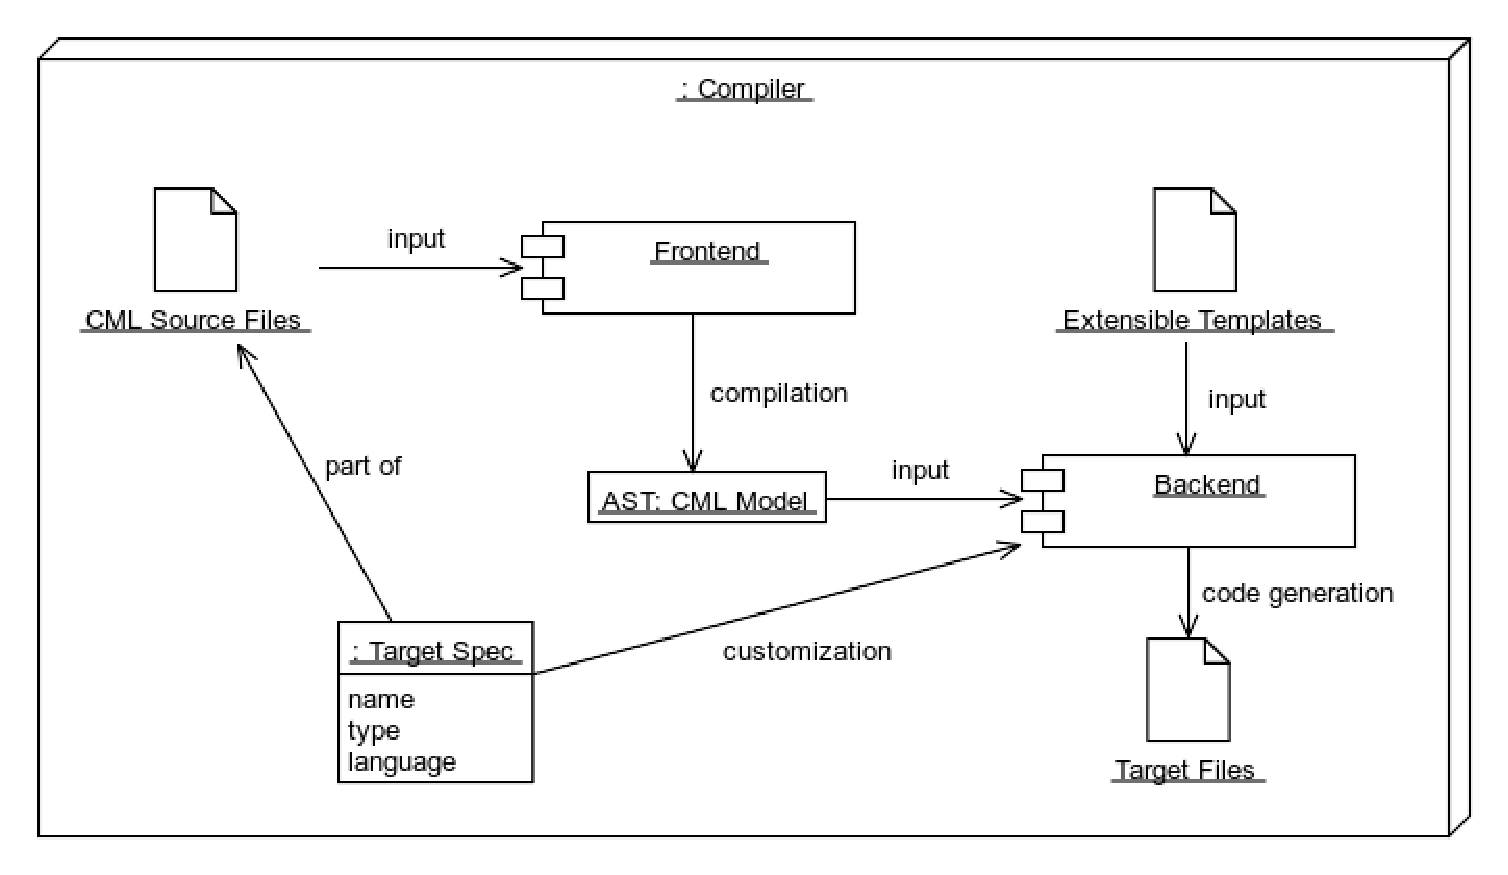
\includegraphics[width=\textwidth]{compiler/figure-overview}
\caption{An architectural overview of the CML compiler.}
\label{fig:overview}
\end{figure}

The CML compiler's overall architecture follows the standard compiler design literature \cite{torben}. An overview diagram of the architecture is shown in figure \ref{fig:overview}.
The two main components of the compiler,
and the artifacts they work with,
are presented in the next sections.
